\section{Ejercicio 2}

En el presente ejercicio se ejecutó el siguiente programa.

\lstinputlisting[language={[Motorola68k]Assembler}]{code/ej2.asm} 

Teniendo en cuenta que los registros parten desde los siguientes estados iniciales:

$$ a = \$00000000000000 $$
$$ b = \$00000000000000 $$
$$ x = \$000000000000 $$

\begin{table}[H]
\centering
\begin{tabular}{|c|c|c|}
\hline
\textbf{Instrucción} & \textbf{Cambios}                                                                                       & \textbf{Comentarios}                                                                                                                                                            \\ \hline
-                  & \begin{tabular}[c]{@{}c@{}}a = \$00000000000000\\ y = \$00000000000000\\ x = \$000000000000\end{tabular} & Carga inicial de valores                                                                                                                                                        \\ \hline
move \#\$caba00, x1         & x = \$caba00000000                                                                                  & \begin{tabular}[c]{@{}c@{}}Se modifica el valor del registro x1 con el valor caba00 \\ por lo que x resulta modificado al valor mostrado.\end{tabular}    \\ \hline
move x1,a                & a = \$ffcaba00000000                                                                                   & \begin{tabular}[c]{@{}c@{}}Se mueve x1 al registro a como el valor \\ caba empieza en 1 (base decimal) se completa \\ con ff (base hexadecimal) hacia adelante.\end{tabular}                                                                       \\ \hline
move x1, b1         & b = \$00caba00000000                                                                                   & \begin{tabular}[c]{@{}c@{}}En este caso el valor del registro x1 se guarda en el b1 \\por lo que b2 y b0 no se ven afectadas por este cambio \\(a diferencia de lo que hubiera pasado si \\guardábamos en el valor de x1 en b).\end{tabular} \\ \hline
\end{tabular}
\caption{Paso a paso de las instrucciones ejecutadas.}
\label{tab:ej2_inst_table}
\end{table}


En la tabla~\ref{tab:ej2_results} se muestra el estado final de los registros.

\begin{table}[H]
\centering
\begin{tabular}{|c|c|c|}
\hline
\textbf{Registro} & \textbf{Valor inicial} & \textbf{Valor final}  \\ \hline
x                 & \$000000000000         & \$caba00000000        \\ \hline
a                 & \$00000000000000       & \$ffcaba00000000      \\ \hline
b                 & \$00000000000000       & \$00caba00000000      \\ \hline
\end{tabular}
\caption{Estado inicial y final de los registros.}
\label{tab:ej2_results}
\end{table}

Se adjunta el estado final de los registros simulados.

\begin{figure}[H]
    \centering
    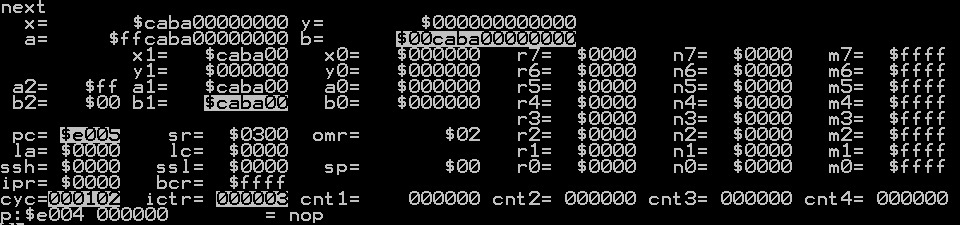
\includegraphics[width=\textwidth]{figs/ej2/ej2_2.jpeg}
    \caption{Estado final de los registros (simulación).}
    \label{fig:ej2_simregs}
\end{figure}
